\chapter{問題}
\label{issue}
% この研究が解く問題をシャープに記述する

本章では、サービス利用者がインターネットサービスを利用する際に利用規約を読む場面において、本研究の解決する問題について述べる。また、利用規約が読まれないことに対しての問題点や原因を明確化した後に、問題解決のための要件を述べる。

\section{利用規約の認知}
2020年に消費者庁が「デジタル・プラットフォーマーの取引慣行等に関する実態調査」の一環として、デジタル広告分野についての実態調査を行い、検索サービス及びSNSの利用者向け(消費者向け)アンケート調査を行った。この調査の結果を以下に示す。
\begin{figure}[h]
  \begin{center}
      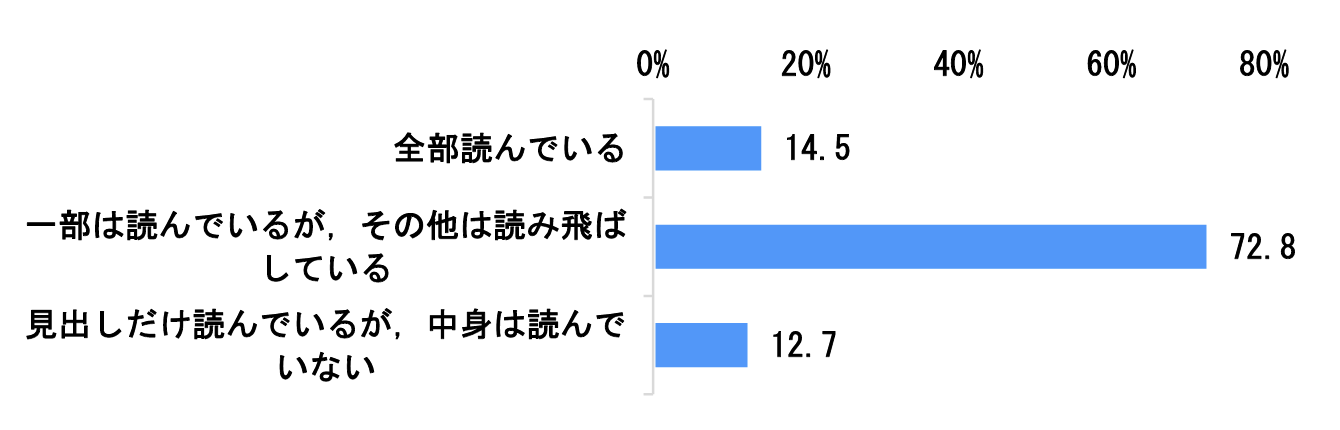
\includegraphics[width=13cm]{img/searchtosyomu.png}
      \caption{検索サービスの利用規約をどの程度読んでいるか(回答数:448)、文献\cite{jftc2021} より引用}
      \label{img:searcjtosyomu}
      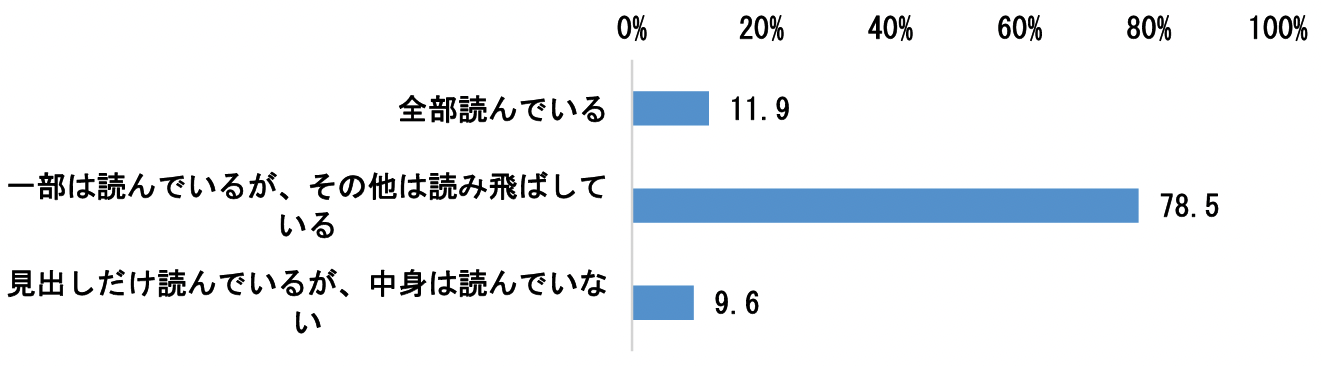
\includegraphics[width=13cm]{img/snstosyomu.png}
      \caption{SNS 等の利用規約をどの程度読んでいるか(回答数:929)、文献\cite{jftc2021} より引用}
      \label{img:snstosyomu}
  \end{center}
\end{figure}

図\ref{img:searcjtosyomu}、\ref{img:snstosyomu}では、それぞれ検索サービス、SNSについて「どの程度読んでいるか」についての調査が行われている。なお、この質問の前段では、「利用規約を認知しているか」についての質問があり、これについて「知っている」を選択した人がこの質問に回答している。このような調査では一般的に、社会適応バイアスにより高めの数値となってしまうことが多いが、それを指し引かなくとも、ほとんどの人が読み飛ばしているもしくは読んでいないという結果が示されている。

\begin{figure}[h]
  \begin{center}
      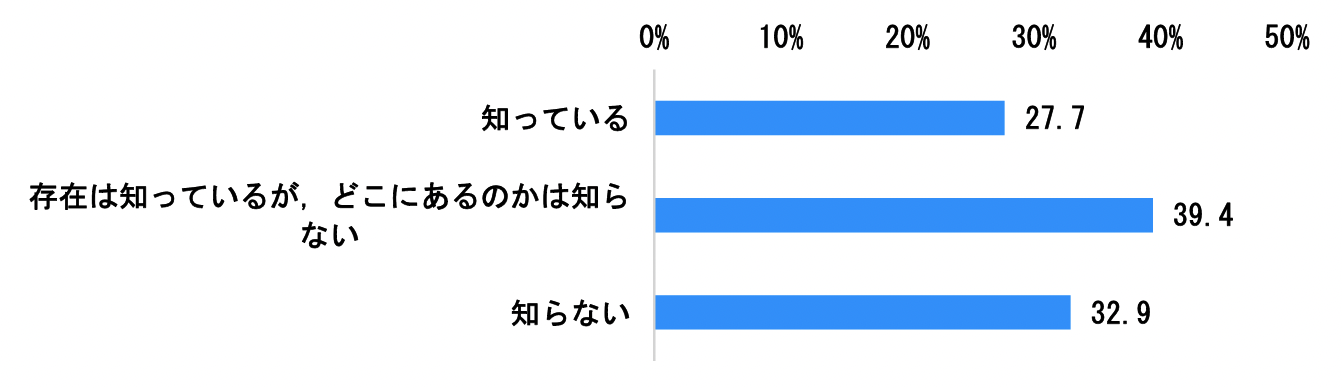
\includegraphics[width=13cm]{img/searchtosninchi.png}
      \caption{検索サービスの利用規約の認知(回答数:2,000)、文献\cite{jftc2021} より引用}
      \label{img:searchtosninchi}
      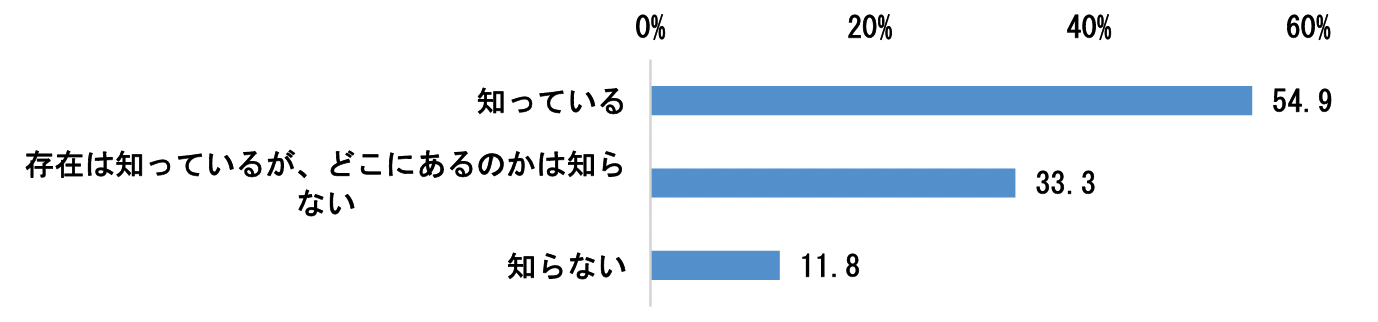
\includegraphics[width=13cm]{img/snstosninchi.png}
      \caption{SNS 等の利用規約の認知(回答数:2,000)、文献\cite{jftc2021}  より引用}
      \label{img:snstosninchi}
  \end{center}
\end{figure}

本研究では、「利用規約の認知」についてはアプローチが非常に困難であることから、この認知を前提として、「利用規約を読み飛ばしてしまう」事象を問題として定義し、それに対するアプローチについての検討を行う。

\section{利用規約の読解}
オムリ・ベン=シャハーほか(2022)\cite{sonokiyaku2022}は、利用規約をはじめとして、食品表示ラベル、著作権表示警告、金融機関の取引前リスク告知、医療行為の場面で行われるインフォームドコンセントなど、法令などで規制されている同意を求める行為をまとめて「開示主義」と定義し、これらの規制を「義務的情報開示」と定義している。その中で、開示主義が失敗していると述べている。(要追記)

\section{問題の定義}
先述したように、利用規約が読まれていないという問題がある。このことは、インターネット上でのサービスを利用する際に、利用規約に関して十分な理解を持っていないままサービスの利用を開始してしまうことになる。これにより、将来的に問題が発生する可能性を孕んだまま利用を継続することになる。この理由の1つとして、利用規約を集中して読むために必要な時間が長すぎる点が挙げられる。本研究では、そのようなユーザーに利用規約を読むことができるように利用規約の読解時間に要する時間が長いということを問題定義とする。

%\section{問題解決の要件}
